\subsection{Type models}
\label{subsec:formalisations:ecore_formalisation:type_models}
This section provides the formal definition of type models, which are models that are based on the Ecore metamodel, of which a simplified version is given in \cref{fig:formalisations:ecore_formalisation:ecore}. A type model provides a set of definitions and constraints that describe a set of instance models, which may or may not be valid according to the type model. On the top level, it defines a set of \textit{classes}, \texttt{EClass}es, of which instances (\textit{objects}) may be used within the instance model. The classes contain a set of \textit{fields}, \texttt{EStructuralFeature}s, which are identified by a name which is unique within the class. Each of these \texttt{EStructuralFeature}s is typed and has a multiplicity. Class instances in the instance model may assign values to these fields (specific for that instance) which must adhere to both the type and multiplicity of the field. The type model also defines an \textit{inheritance} relation between these classes, modelled by \texttt{eSupertypes} in the Ecore metamodel, which allows classes to inherit from other classes, providing a specialisation of that class.

A type model also defines a set of \textit{enumerations}, \texttt{EEnum}s, and their values, \texttt{EEnumLiteral}s. Each enumeration defines a unique type with a fixed set of values. Furthermore, a set of \textit{constants} and their types define a symbolic typed value, which relates to a specific value in an instance model. A set of \textit{custom data types}, \texttt{EDataType}s, is also provided by the type model, which allows the representation of user-defined data types.

Finally, a set of \textit{properties} of the type model specifies the properties an instance model of this type model has to satisfy in order to be valid. These properties specify constraints on the values and structure of such an instance model.

The definition of a type model depends on the definition of various types. These types again depend on the definition of the type model. The solution to this cyclic dependency is the smallest solution to the set of equations given for the types and type model.

The suffix $Tm$ is used when the definition of something depends on any type model $Tm$, for example, $Class_{Tm}$.

\begin{defin}[Type model]
\label{defin:formalisations:ecore_formalisation:type_models:type_model}
A single type model $Tm$ is a 10-tuple, consisting of 8 sets and 2 functions, which is defined as:
\begin{equation*}
    Tm = \langle Class, Enum, UserDataType, Field, \mathrm{FieldSig}, EnumValue, Inh, Prop, Constant, \mathrm{ConstType} \rangle
\end{equation*}
with
\begin{itemize}
    \item $Class \subseteq Id$ is the set of classes (\texttt{EClass} objects) in $Tm$.
    \item $Enum \subseteq Id$ is the set of enumerations (\texttt{EEnum} objects) in $Tm$.
    \item $UserDataType \subseteq Id$ is the set of custom data types (\texttt{EDataType} objects) in $Tm$.
    \item $Field \subseteq (Class \times Name)$ is the set that maps a class to a set of field names (\texttt{EStructuralFeature} objects) in $Tm$.
    \item $\mathrm{FieldSig}: Field \Rightarrow (Type_{Tm} \times \mathbb{M})$ is the function that maps fields to their type (as defined in \cref{defin:formalisations:ecore_formalisation:type_models:types}) and multiplicity (as defined in \cref{defin:formalisations:global_definitions:multiplicity}).
    \item $EnumValue \subseteq Enum \times Name$ is the set of possible values (the \texttt{EEnumLiteral}s) for the enumerations in $Tm$.
    \item $Inh \subseteq Class \times Class$ is the inheritance relation between the classes in $Tm$.
    \item $Prop \subseteq Property_{Tm}$ is the set of properties that apply to $Tm$ (see definition \cref{defin:formalisations:ecore_formalisation:type_models:type_model_properties}).
    \item $Constant \subseteq Id$ is the set that contains all possible constants that may be used as a (symbolic) default value.
    \item $\mathrm{ConstType}: Constant \Rightarrow Type_{Tm}$ is the function that maps constants to their respective types.
\end{itemize}
where
\begin{itemize}
    \item $Class$, $DataType$ (\cref{defin:formalisations:ecore_formalisation:definitions:data_types}), $Enum$ and $UserDataType$ are pairwise disjoint.
    \item None of the elements in $Class \cup DataType \cup Enum \cup UserDataType$ may be in the namespace of another element in that set.
    \item $Inh$ is an asymmetric relation, of which the transitive closure is irreflexive.
\end{itemize}

\isabellelref{type_model}{Ecore.Type_Model}
\end{defin}

\begin{figure}[p]
    \centering
    \begin{subfigure}{\textwidth}
        \centering
        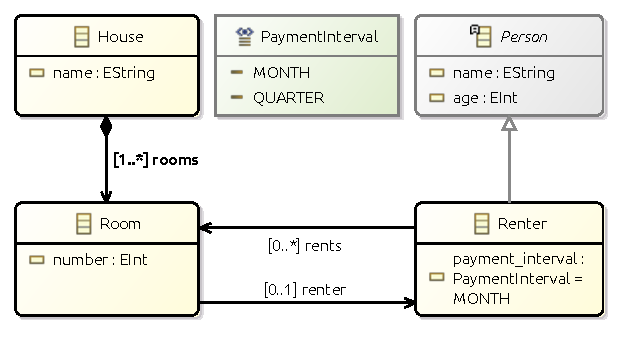
\includegraphics{images/03_formalisations/02_ecore_formalisation/type_model_example.pdf}
        \caption{Type model in Ecore notation}
    \end{subfigure}
    
    \begin{subfigure}{\textwidth}
        \centering
        \begin{align*}
            Class_{Tm} =\ & \{ 
                .\type{House}, 
                .\type{Person}, 
                .\type{Renter}, 
                .\type{Room} 
            \}\\
            Enum_{Tm} =\ & \{ 
                .\type{PaymentInterval} 
            \}\\
            UserDataType_{Tm} =\ & \emptyset\\
            Field_{Tm} =\ & \{ 
                ( .\type{House}, \type{name} ),
                ( .\type{House}, \type{rooms} ),\\&
                ( .\type{Person}, \type{age} ), 
                ( .\type{Person}, \type{name} ),\\&
                ( .\type{Renter}, \type{payment\_interval} ),
                ( .\type{Renter}, \type{rents} ),\\&
                ( .\type{Room}, \type{number} ),
                ( .\type{Room}, \type{renter} )
            \}\\
            \mathrm{FieldSig}_{Tm} =\ & \Big\{ 
                \Big( \big( .\type{House}, \type{name} \big), \big( \type{string}, 1..1 \big) \Big),
                \Big( \big( .\type{House}, \type{rooms} \big), \big( [ \type{setof},  !.\type{Room} ], 1..\mstar \big) \Big),\\&
                \Big( \big( .\type{Person}, \type{age} \big), \big( \type{integer}, 1..1 \big) \Big), 
                \Big( \big( .\type{Person}, \type{name} \big), \big( \type{string}, 1..1 \big) \Big),\\&
                \Big( \big( .\type{Renter}, \type{payment\_interval} \big), \big( .\type{PaymentInterval}, 1..1 \big) \Big),\\&
                \Big( \big( .\type{Renter}, \type{rents} \big), \big( [ \type{setof}, !.\type{Room} ], 0..\mstar \big) \Big),\\&
                \Big( \big( .\type{Room}, \type{number} \big), \big( \type{integer}, 1..1 \big) \Big),
                \Big( \big( .\type{Room}, \type{renter} \big), \big( !.\type{Renter}, 0..1 \big) \Big)
            \Big\}\\
            EnumValue_{Tm} =\ & \{ 
                ( .\type{PaymentInterval}, \type{MONTH} ),
                ( .\type{PaymentInterval}, \type{QUARTER} )
            \}\\
            Inh_{Tm} =\ & \{ 
                ( .\type{Renter}, .\type{Person} )
            \}\\
            Prop_{Tm} =\ & \{ 
                [ \type{abstract}, .\type{Person} ], \\&
                [ \type{identity}, \{( .\type{Person}, \type{age} ), ( .\type{Person}, \type{name} )\} ],
                [ \type{containment}, ( .\type{House}, \type{rooms} ) ],\\&
                [ \type{opposite}, ( .\type{Room}, \type{renter} ), ( .\type{Renter}, \type{rents} ) ], 
                [ \type{opposite}, ( .\type{Renter}, \type{rents} ), ( .\type{Room}, \type{renter} ) ],\\&
                [ \type{defaultValue}, ( .\type{Renter}, \type{payment\_interval} ), .\type{Constant}.\type{PaymentInterval}.\type{Month} ]
            \}\\
            Constant_{Tm} =\ & \{ 
                .\type{Constant}.\type{PaymentInterval}.\type{Month}
            \}\\
            \mathrm{ConstType}_{Tm} =\ & \{ 
                ( .\type{Constant}.\type{PaymentInterval}.\type{Month}, .\type{PaymentInterval} )
            \}
        \end{align*}
        \caption{Formal definition of the type model}
    \end{subfigure}
    \caption{Example of a type model corresponding with \cref{defin:formalisations:ecore_formalisation:type_models:type_model}}
    \label{fig:formalisations:ecore_formalisation:type_models:type_model_example}
\end{figure}

An example type model is given in \cref{fig:formalisations:ecore_formalisation:type_models:type_model_example}. It shows 4 classes ($\type{House}$, $\type{Person}$, $\type{Renter}$ and $\type{Room}$) and a single enumeration ($\type{PaymentInterval}$). The $\type{Person}$ class has 2 fields, $\type{age}$ and $\type{name}$. The $\type{Renter}$ class has a field $\type{payment\_interval}$ which makes use of the $\type{PaymentInterval}$ enumeration. It also has a field $\type{rents}$ which defines a relation between $\type{Room}$ and $\type{Renter}$. The $\type{House}$ class has also 2 fields, a field $\type{name}$ and a field $\type{rooms}$ which is a containment relation between $\type{House}$ and $\type{Room}$. Moreover, we have the $\type{Room}$ class itself, which has 2 fields. One is called $\type{number}$ and the other one is called $\type{renter}$, which is the opposite relation between $\type{Room}$ and $\type{Renter}$. Finally, we see that $\type{Renter}$ inherits from $\type{Person}$.

The fields in a type model are always associated with a specific type, which defines the set of possible values that may be assigned in an instance model. The possible types are defined by the set of data types, classes, enumerations and user-defined data types. The set of types also consists of various aggregations of these types, namely containers. Containers provide types for multiple values of the same type, but of which the values may differ in number and order.

\begin{defin}[Types]
\label{defin:formalisations:ecore_formalisation:type_models:types}
Given any type model $Tm$, the set of types is defined as
\begin{equation*}
Type_{Tm} = DataType \cup ClassType_{Tm} \cup Enum_{Tm} \cup UserDataType_{Tm} \cup Container_{Tm}
\end{equation*}

The $ClassType_{Tm}$ set defines both a set of nullable and proper classes. Nullable classes are classes for which the $\type{nil}$ (see \cref{defin:formalisations:ecore_formalisation:definitions:nil}) value is valid, and proper classes are those classes for which the $\type{nil}$ value is not valid (hence both sets of classes are disjoint). 

The $ClassType_{Tm}$ set is defined as
\begin{equation*}
ClassType_{Tm} = \{ \type{nullable}, \type{proper} \} \times Class_{Tm}
\end{equation*}

A container is a type that may contain multiple values in an instance. Containers define the type of values they contain, and the multiplicity of the container. They are defined by 
\begin{equation*}
Container_{Tm} = \{ \type{bagof}, \type{setof}, \type{seqof}, \type{ordof} \} \times Type_{Tm}
\end{equation*}
For the interpretation of the values in $\{ \type{bagof}, \type{setof}, \type{seqof}, \type{ordof} \}$, see \cref{defin:formalisations:ecore_formalisation:instance_models:values}.

The set of types is recursively defined as the smallest solution of the equations for $Type_{Tm}$ and $Container_{Tm}$.

Tuples within $Type_{Tm}$ are written using square brackets, e.g. $[\type{bagof}, \type{int} ]$ or $[ \type{nullable}, C ]$. Furthermore, given a $C \in Class_{Tm}$, $?C$ is a short notation for the $\type{nullable}$ variant of $C$, $[ \type{nullable}, C ]$. In the same fashion, $!C$ is the short notation for the $\type{proper}$ variant of $C$, $[ \type{proper}, C ]$.

Finally, we define the function $\mathrm{uncontainer}\!: Container_{Tm} \Rightarrow Type_{Tm}$ which returns the type contained by a container.

\isabellelref{Type}{Ecore.Type_Model}
\end{defin}

In the example in \cref{fig:formalisations:ecore_formalisation:type_models:type_model_example}, the various fields make use of different types. The fields depicted as a relation between two classes are actually of a type based on the $Class_{Tm}$ set. For example, the $\type{rooms}$ field of class $\type{House}$ is typed by the $\type{Room}$ class. In this case, we assume that each $\type{Room}$ in a $\type{House}$ is unique. Thus the relationship is best typed by a $\type{setof}$ container. For a $\type{setof}$ container, the order does not matter, and each value should be unique. We also see the example of the usage of an enumeration, the $\type{payment\_interval}$ field on $\type{Renter}$ uses the $\type{PaymentInterval}$ enumeration. Finally, the $\type{Person}$ class shows two fields that are typed by some of the data types available, integer and string for the age and name fields respectively.

\begin{defin}[Field]
\label{defin:formalisations:ecore_formalisation:type_models:field}
Given any type model $Tm$, the $Field_{Tm}$ relation defines a binary relation between classes and fields.
In order to retrieve the set of fields for a given class (and the fields inherited from superclasses), the following function is defined:
\begin{equation*}
   \mathrm{fields}\!: Class_{Tm} \Rightarrow \mathcal{P}(Field_{Tm})
\end{equation*}
such that
\begin{equation*}
\mathrm{fields}_{Tm}(c) = \{f \in Field_{Tm} \mid f = ( c', n ) \land c \sqsubseteq_{Tm} c'\}
\end{equation*}

Given any type model $Tm$, the $\mathrm{FieldSig}_{Tm}$ function defines a mapping between fields and their signatures. The following functions are defined to retrieve various components of a field signature:
\begin{itemize}
    \item $\mathrm{class}\!: Field_{Tm} \Rightarrow Class_{Tm}$
    \item $\mathrm{type}\!: Field_{Tm} \Rightarrow Type_{Tm}$
    \item $\mathrm{lower}\!: Field_{Tm} \Rightarrow \mathbb{N}$
    \item $\mathrm{upper}\!: Field_{Tm} \Rightarrow \mathbb{N}^+ \cup {\mstar}$
\end{itemize}
These functions are defined as follows:
\begin{itemize}
    \item $\mathrm{class}_{Tm}(f) = class \quad \mathrm{iff} \quad f = ( class, name)$
    \item $\mathrm{type}_{Tm}(f) = type \quad \mathrm{iff} \quad \mathrm{FieldSig}_{Tm}(f) = ( type, ( lower, upper ) )$
    \item $\mathrm{lower}_{Tm}(f) = lower \quad \mathrm{iff} \quad \mathrm{FieldSig}_{Tm}(f) = ( type, ( lower, upper ) )$
    \item $\mathrm{upper}_{Tm}(f) = upper \quad \mathrm{iff} \quad \mathrm{FieldSig}_{Tm}(f) = ( type, ( lower, upper ) )$
\end{itemize}

Fields can be separated into relation and attribute sets, where attributes reference (containers of) data types, user data types and enumerations, and relations reference all other types. The sets are defined by
\begin{align*}
    Attr_{Tm} =&\, \{f \in Field_{Tm} \mid type(f) \in (DataType \cup Enum_{Tm} \cup UserDataType_{Tm})\,\vee\\&\quad type(f) \in \{ \type{setof}, \type{bagof}, \type{ordof}, \type{seqof} \} \times Attr_{Tm}\}\\
    Rel_{Tm} =&\, Field_{Tm} \setminus Attr_{Tm}
\end{align*}
The set of attributes is recursively defined as the smallest solution of the given set of equations for $DataType$, $Enum_{Tm}$, $UserDataType_{Tm}$ and $Attr_{Tm}$

\isabellelref{fields}{Ecore.Type_Model}
\end{defin}

Taking for example the field $\type{rents}$ from the $\type{Renter}$ class in the type model example in \cref{fig:formalisations:ecore_formalisation:type_models:type_model_example}, the following properties can be identified: The type refers to $\type{Room}$, which is an element of the $Class_{Tm}$ set. The
lower and upper values are $0$ and $\mstar$ respectively (which means a $\type{Renter}$ can rent an arbitrary number of rooms). Furthermore, the $\type{rents}$ field is an element of the $Rel_{Tm}$ set (it is a class container type) and part of the $fields_{Tm}(\type{Renter})$ set, which is $\{ \type{payment\_interval}, \type{rents} \}$.

The various types have an underlying subtype relation, which generalises inheritance. A subtype defines a specialisation of a supertype. Because of that, all values valid for the subtype are also valid for the supertype (see \cref{defin:formalisations:ecore_formalisation:instance_models:valid_type_values} for details).

\begin{defin}[Subtype relation]
\label{defin:formalisations:ecore_formalisation:type_models:subtype_relation}
Given any type model $Tm$, $\sqsubseteq_{Tm}\, \subseteq Type_{Tm} \times Type_{Tm}$ defines the subtype relation. It is a reflexive partial order relation, for which the following rules
can be defined (with $t_1, t_2, t_3 \in Type_{Tm}$ and $c_1, c_2 \in Class_{Tm}$):

Transitivity:
\begin{mathpar}
    \inferrule{t_1 \sqsubseteq_{Tm} t_2 \\ t_2 \sqsubseteq_{Tm} t_3}{t_1 \sqsubseteq_{Tm} t_3}
\end{mathpar}

Reflexivity:
\begin{mathpar}
    \inferrule{\ }{t_1 \sqsubseteq_{Tm} t_1}
\end{mathpar}

Generalization of inheritance:
\begin{mathpar}
    \inferrule{(c_1, c_2) \in Inh_{Tm}}{?c_1 \sqsubseteq_{Tm}\: ?c_2}
    \and
    \inferrule{(c_1, c_2) \in Inh_{Tm}}{!c_1 \sqsubseteq_{Tm}\: !c_2}
\end{mathpar}

Nullable/Proper classes:
\begin{mathpar}
    \inferrule{\ }{!c_1 \sqsubseteq_{Tm}\: ?c_1}
\end{mathpar}

\isabellelref{subtype}{Ecore.Type_Model}
\end{defin}

Thus, in the example, $[ \type{nullable}, \type{Renter} ] \sqsubseteq_{Tm} [ \type{nullable}, \type{Person} ]$ (since $(\type{Student}, \type{Person}) \in Inh_{Tm}$). Furthermore, it also holds that $[ \type{proper}, \type{Renter} ] \sqsubseteq_{Tm} [ \type{nullable}, \type{Renter} ]$, as a proper class is a subtype of a nullable class.

A type model may specify a set of properties, $Prop$, which an instance model has to satisfy in order to be valid. The following properties are defined:
\begin{itemize}
\item The $\type{abstract}$ property. This property, specified for a specific class in the type model, forbids the instantiation of that class in any instance model. As such, it is satisfied when no object exists in an instance model which is an instance of that class. Please note that this only holds for instances of that exact class. Subtyping may be allowed (under the condition that those classes are not $\type{abstract}$).

\item The $\type{containment}$ property. This property, specified for a relation, states that a single source object contains all objects that are the target of this relation. Objects are contained by at most one other object, and containment cycles are not allowed. When an object with contained objects is removed from an instance model, all contained objects are removed as well. The constraint is satisfied when an object is the target of no more than one containment relation, and there exists no cycle between containment relations.

\item The $\type{defaultValue}$ property. This property specifies a default value for a field which has not been assigned a value in an instance model. It specifies a constant for a field, which represents a value in an instance model. It is always satisfied and influences the behaviour of possible model transformations.

\item The $\type{identity}$ property. This property is specified for a class and a set of attributes. It is used to specify that the values for the set of attributes uniquely identify an object on instance model level. As such, it is satisfied when no two objects are both an instance of the class and have pairwise the same value for all the attributes.

\item The $\type{keyset}$ property. This property is specified for a set of attributes of a class and a relation towards that class. It ensures that each instance of that class within the given relation is uniquely identified by the values of the set of attributes. It is satisfied that two objects must be the same object if they are the target of the given relation, and they have pairwise-identical values for their attributes.

\item The $\type{opposite}$ property. This property specifies that two relations are the opposite of each other, which means that for each instance of the first relation, an instance of the second relation exists with a switched target and source. The property is satisfied when for each pair of objects, for each relation that exists between these objects, a reverse relation exists if both these relations are opposite.

\item The $\type{readonly}$ property. This property, specified for a field in the type model, forbids the assignment of a new value to that field in any instance model. This property only affects the possible transformations of an instance model and is always satisfied for any specific instance model.
\end{itemize}

\begin{defin}[Type model properties]
\label{defin:formalisations:ecore_formalisation:type_models:type_model_properties}
For a type model $Tm$ a set of properties $Property_{Tm}$ is defined which contains all the possible properties. This set is defined as 

\begin{align*}
    Property_{Tm} =\ &
    \{[ \type{abstract}, c ] \mid c \in Class_{Tm} \}\ \cup \\&
    \{[ \type{containment}, r ] \mid r \in Rel_{Tm} \}\ \cup \\&
    \{[ \type{defaultValue}, f, v ] \mid f \subseteq Field_{Tm} \land v \in Constant_{Tm} \}\ \cup \\&
    \{[ \type{identity}, c, A ] \mid c \in Class_{Tm} \land A \subseteq Attr_{Tm} \}\ \cup \\&
    \{[ \type{keyset}, r, A ] \mid r \in Rel_{Tm} \land A \subseteq Attr_{Tm} \}\ \cup \\&
    \{[ \type{opposite}, r, r' ] \mid r, r' \subseteq Rel_{Tm} \land r \not= r'\}\ \cup \\&
    \{[ \type{readonly}, f ] \mid f \in Field_{Tm} \}
\end{align*}

where
\begin{itemize}
    \item $[ \type{defaultValue}, f, v ]$ is defined such that $\mathrm{ConstType}_{Tm}(v) \sqsubseteq_{Tm} \mathrm{type}_{Tm}(f)$.
    \item $[ \type{keyset}, r, A ]$ is defined such that $\mathrm{type}_{Tm}(r) \in (\{ \type{setof}, \type{ordof} \} \times ClassType_{Tm})$ with $\mathrm{type}_{Tm}(r) = [\type{setof}, c] \lor \mathrm{type}_{Tm}(r) = [ \type{ordof}, c ]$. Then also have that $\forall ( ac, an ) \in A\!:\: !c\sqsubseteq_{Tm}\,!ac$.
    \item $[ \type{opposite}, r, r' ]$ is defined such that when $r = ( c1, n1 ), r' = ( c2, n2 )$, then it should hold that $!c1 \sqsubseteq_{Tm} \mathrm{uncontainer}(\mathrm{type}_{Tm}(r'))$, $!c2 \sqsubseteq_{Tm} \mathrm{uncontainer}(\mathrm{type}_{Tm}(r))$, $\mathrm{type}_{Tm}(r) \not\in \{ \type{bagof}, \type{seqof} \} \times Type_{Tm}$ and finally $type_{Tm}(r') \not\in \{ \type{bagof}, \type{seqof} \} \times Type_{Tm}$ (containers must have unique values).
\end{itemize}

\isabellelref{Property}{Ecore.Type_Model}
\end{defin}

The example in \cref{fig:formalisations:ecore_formalisation:type_models:type_model_example} also shows a few properties:
\begin{itemize}
    \item The $\type{Person}$ class is declared abstract (indicated by the grey looking class layout and italic name)
    \item The $\type{age}$ and $\type{name}$ fields of a $\type{Person}$ are its identity (as indicated by the formal definition). Although it is highly unlikely that these details would be unique in the real world, they must be in our instance models.
    \item The $\type{rooms}$ relation of $\type{House}$ is a containment relation (shown by the filled diamond at the $\type{House}$ end of the containment relation).
    \item The $\type{rents}$ and $\type{renter}$ relations are opposites (as indicated by the formal definition).
    \item The $\type{payment\_interval}$ field has a default value $\type{MONTH}$ (as indicated with the field definition in the model).
\end{itemize}

With the given definitions, it is possible to define an inconsistent type model. Such a type model is correct according to the given definitions but does not specify any valid instance model using the definitions in \cref{subsec:formalisations:ecore_formalisation:instance_models}. Therefore, a definition is given for a consistent type model. A consistent type model enforces some constraints on multiplicities and properties within the type model to ensure the satisfiability of the definitions in \cref{subsec:formalisations:ecore_formalisation:instance_models}. Without these constraints, one or more of these definitions can never be satisfied at all. Please note that these constraints merely support the satisfiability of these definitions, it does not guarantee the existence of any meaningful instance model, as it might still be possible to define a `consistent' type model with conflicting multiplicities or properties.

\begin{table}[t]
    \centering
    \rowcolors{2}{gray!25}{white}
    \begin{tabular}{l|l}
        \rowcolor{gray!50}
        $Type_{Tm}$ & Multiplicity\\
        $\{ \type{proper} \} \times Class_{Tm}$ & $1..1$\\
        $\{ \type{nullable} \} \times Class_{Tm}$ & $0..1$\\
        $Container_{Tm}$ & $x..y \: (0 \leq x \leq y \land 1 \leq y)$\\
        $DataType$ & $1..1$\\
        $Enum_{Tm}$ & $1..1$\\
        $UserDataType_{Tm}$ & $1..1$
    \end{tabular}
    \caption{The allowed multiplicities for each type}
    \label{tab:formalisations:ecore_formalisation:type_models:possible_multiplicities}
\end{table}

\begin{defin}[Type model consistency]
\label{defin:formalisations:ecore_formalisation:type_models:type_model_consistency}
The multiplicities of the fields in $Field_{Tm}$ are consistent if it holds that:
\begin{align*}
    \mathrm{type}_{Tm}(f) \in DataType \cup Enum_{Tm} \cup UserDataType_{Tm} \cup (\type{proper} \times Class_{Tm}) \implies & \mathrm{lower}_{Tm}(f) = 1 \\
    \mathrm{type}_{Tm}(f) \in (\type{nullable} \times Class_{Tm}) \implies & \mathrm{lower}_{Tm}(f) = 0
\end{align*}
and
\begin{align*}
    \mathrm{type}_{Tm}(f) \not\in Container_{Tm} \implies & \mathrm{upper}_{Tm}(f) = 1
\end{align*}
as indicated by \cref{tab:formalisations:ecore_formalisation:type_models:possible_multiplicities}.

The properties in $Prop_{Tm}$ are consistent if the following holds:
\begin{itemize}
    \item $[ \type{containment}, r ] \in Prop_{Tm} \land [ \type{opposite}, r, r' ] \in Prop_{Tm} \Longrightarrow upper_{Tm}(r') = 1$ (opposite of containment relation must have upper bound of 1).
    \item $[ \type{defaultValue}, f, v ] \in Prop_{Tm} \land [ \type{defaultValue}, f, v' ] \in Prop_{Tm} \Longrightarrow v = v'$ (unique for f).
    \item $[ \type{identity}, c_1, A_1 ] \in Prop_{Tm} \land [ \type{identity}, c_2, A_2 ] \in Prop_{Tm}\: \land\: !c_1 \sqsubseteq_{Tm}\, !c_2 \Longrightarrow A_1 \subseteq A_2$ (classes may only have identities with attributes that are a subset of attributes part of the superclass' identity).
    \item $[ \type{keyset}, r, A ] \in Prop_{Tm} \land [ \type{keyset}, r, A' ] \in Prop_{Tm} \Longrightarrow A = A'$ (unique for $r$).
    \item $[ \type{opposite}, r, r' ] \in Prop_{Tm} \land [ \type{opposite}, r, r'' ] \in Prop_{Tm} \Longrightarrow r' = r''$ (unique for r).
    \item $[ \type{opposite}, r, r' ] \in Prop_{Tm} \Longleftrightarrow [ \type{opposite}, r', r ] \in Prop_{Tm}$ (symmetry).
\end{itemize}

Then a type model $Tm$ is consistent if and only if
\begin{itemize}
\item The multiplicities of all fields in $Field_{Tm}$ are consistent.
\item All properties in $Prop_{Tm}$ are consistent.
\end{itemize}

\isabellelref{type_model}{Ecore.Type_Model}
\end{defin}